\section{Set theory}

% Offering-specific handouts may begin immediately after Proposition 1.67.
% Preserve the theorem and subsection numbering from the master notes.
\ifdefined\startaftercountableproduct
  \setcounter{theorem}{67}
  \setcounter{subsection}{5}
\else

% Offering-specific handouts may begin at Section 1.4 without duplicating
% the canonical source. Preserve the theorem numbering from the master notes.
\ifdefined\startataxiomofchoice
  \setcounter{theorem}{43}
  \setcounter{subsection}{3}
\else

In this section we review/develop the set‑theoretic background for the course.

\subsection{Basic definitions}
Naive definition: A set is an aggregate of things, called \emph{elements} of the set.  We usually use capital letters to denote sets, such as $A$, $B$, $C$, and lowercase letters for elements, such as $a$, $b$, $c$.  The notation \(a\in A\) means that $a$ is an element of the set $A$. We write $a\notin A$ to mean that $a$ is not an element of the set $A$.

\begin{example}
Some basic examples of sets include:
\begin{itemize}
\item The natural numbers $\mathbb{N} = \{1, 2, 3, \ldots\}$
\item The integers $\mathbb{Z} = \{\ldots, -2, -1, 0, 1, 2, \ldots\}$
\item The real numbers $\mathbb{R}$
\end{itemize}
\end{example}



\paragraph{Set calculus}
A set $A$ is a subset of a set $B$ if every element of $A$ is also an element of $B$.  We write \(A\subseteq B\) to denote that $A$ is a subset of $B$.  If $A$ is a subset of $B$ but not equal to $B$, we say that $A$ is a \emph{proper subset} of $B$ and denote it by \(A\subsetneq B\). 

We let $\mathcal{P}(A)$ denote the \emph{power set} of $A$, which is the set of all subsets of $A$.

We say two sets $A$ and $B$ are \emph{equal} if they have the same elements, that is, if \(A\subseteq B\) and \(B\subseteq A\).  We write \(A=B\) to denote that $A$ and $B$ are equal.

We let $A\backslash B$ denote the \emph{set difference} of $A$ and $B$, which is the set of elements in $A$ that are not in $B$.  Formally, \(A\backslash B = \{x \in A : x \notin B\}\). When $B\subseteq A$, we say $A\backslash B$ is the \emph{complement} of $B$ in $A$.

The empty set, denoted \(\varnothing\), is a set that contains no elements.  It is a subset of every set.




\begin{definition}
A family of sets $\mathcal{A}$ is a set whose elements are sets. Usually, we can write the family of sets as $$\mathcal{A}=\{A_i\}_{i\in I}$$ for some index set $I$. 

If $\mathcal{A}$ is a family of sets, we define the union of the family as
\[\bigcup_{A\in\mathcal{A}} A:=\{x| \exists A\in\mathcal{A}, x\in A\}.\]
and the intersection as
\[\bigcap_{A\in\mathcal{A}} A:=\{x| \forall A\in\mathcal{A}, x\in A\}.\]

\end{definition}

\begin{theorem}
  Let X be a set and $\{A_i\}_{i\in I}\subseteq \mathcal{P}(X)$. Then (De Morgan's laws)
  \[
  X\setminus \biggl(\bigcup_{i\in I} A_i\biggr)=\bigcap_{i\in I}\bigl(X\setminus A_i\bigr),
  \qquad
  X\setminus \biggl(\bigcap_{i\in I} A_i\biggr)=\bigcup_{i\in I}\bigl(X\setminus A_i\bigr).
  \]
  Moreover, for any $A\subseteq X$ and $\{B_i\}_{i\in I}\subseteq \mathcal{P}(X)$ (distributive laws),
  \[
  A\cap \biggl(\bigcup_{i\in I} B_i\biggr)=\bigcup_{i\in I}\bigl(A\cap B_i\bigr),
  \qquad
  A\cup \biggl(\bigcap_{i\in I} B_i\biggr)=\bigcap_{i\in I}\bigl(A\cup B_i\bigr).
  \]
\end{theorem}

\begin{example}[Russell's paradox]
  Let $P$ denote the set of all sets. Then, form $Q:=\{A\in P|A\notin A\}$. Is $Q\in Q$? 
\end{example}

More axiomatic treatment of sets can be found in Zermelo-Fraenkel set theory (ZF), which provides a formal foundation for set theory and avoids paradoxes like Russell's paradox by carefully restricting the kinds of sets that can be formed. For example, under ZF axioms, the collection of all sets is not a set but a \emph{proper class}, because it violates one of the axioms requiring that a set cannot contain itself as an element.



\subsection{Functions}


\paragraph{Cartesian product}

The \emph{Cartesian product} of two sets $A$ and $B$, denoted $A\times B$, is the set of all ordered pairs \((a,b)\) where \(a\in A\) and \(b\in B\):
\[
A\times B = \{(a,b) : a\in A, b\in B\}.
\]

Formally, an ordered pair can be defined as follows and define the cartesian product as a set of sets:
\[
(a,b) := \{\{a\},\{a,b\}\}.
\]

\begin{remark}
  If one set is empty, then the Cartesian product is also empty:
  \[
  A\times \varnothing = \varnothing \times B = \varnothing.
  \]
\end{remark}

\begin{definition}
  A function \(f\colon A\to B\) is a subset of the Cartesian product \(A\times B\) such that for any \(a\in A\), there exists a unique \(b\in B\) such that \((a,b)\in f\).
\end{definition}

Of course, since each $a\in A$ is associated with a unique $b\in B$, we often write \(f(a) = b\) and then
\[
f = \{(a,f(a)) : a\in A\} \subseteq A\times B.
\]

For any $C\subseteq A$, we define the image of $C$ under $f$ as the set 
\[f(C) = \{f(a) : a\in C\}.\]
We call $f(A)$ the \emph{image} of $f$.

For any $D\subseteq B$, we define the preimage of $D$ under $f$ as the set
\[f^{-1}(D) = \{a\in A : f(a)\in D\}.\]

If the image of $f$ is equal to $B$, we say that $f$ is \emph{onto} or \emph{surjective}.  If for any $a_1\neq a_2$ we have that $f(a_1)\neq f(a_2)$, we say that $f$ is \emph{one‑to‑one} or \emph{injective}.  If a function is both injective and surjective, it is called a \emph{bijection}. We usually denote a bijection by $f:A\cong B$.

Let \(f\colon A\to B\) and \(g\colon B\to C\) be two functions.  The \emph{composition} of \(f\) and \(g\) is the function \(g\circ f\colon A\to C\) defined by
\[
(g\circ f)(a) = g(f(a)) \quad \text{for all } a\in A.
\]

\begin{example}
  For any nonempty set $A$, we define the identity function $id_A:A\to A$ by $id_A(a)=a$ for all $a\in A$.  It is clear that $id_A$ is a bijection.  Moreover, for any function $f:A\to B$, we have $f\circ id_A=f$ and $id_B\circ f=f$.
\end{example}




\paragraph{Cartesian products of families of sets}

If $\{A_i\}_{i\in I}$ is a family of sets indexed by a set $I$, the Cartesian product of the family is defined as
\[\prod_{i\in I} A_i = \{f : I\to \bigcup_{i\in I} A_i : f(i)\in A_i \text{ for all } i\in I\}.\]

\begin{example}
  If $I=\{1,2,\ldots,n\}$ is a finite set, then \(\prod_{i\in I} A_i\) can be identified with the set of ordered \(n\)-tuples \((a_1,a_2,\ldots,a_n)\) where \(a_i\in A_i\) for each \(i\).
\end{example}


\subsection{Relations}

\begin{definition}
  
  A \emph{relation} on a set \(S\) is any subset \(R\subseteq S\times S\).  If \((a,b)\in R\), we say that \(a\) is related to \(b\) and write \(aRb\).
  
  A relation \(R\) is called 
  \begin{itemize}
    \item \emph{reflexive} if \(aRa\) for all \(a\in S\);
    \item \emph{symmetric} if \(aRb\) implies \(bRa\);
    \item \emph{transitive} if \(aRb\) and \(bRc\) imply \(aRc\);
    \item \emph{antisymmetric} if \(aRb\) and \(bRa\) imply \(a=b\).
  \end{itemize}
\end{definition}


\subsubsection{Equivalence relations}
\begin{definition}
  We say that \(R\) is an \emph{equivalence relation} if it is reflexive, symmetric, and transitive. An equivalence relation is usually denoted by \(\sim\) and if $(a,b)\in \sim$ we write $a\sim b$.
\end{definition}

\begin{example}
  The relation \(R\) on \(\mathbb{Z}\) defined by \(aRb\) if and only if \(a-b\) is even is an equivalence relation.
\end{example}

\begin{example}
  Let $f:A\to B$ be any function.  The relation \(R\) on \(A\) defined by \(aRb\) if and only if \(f(a)=f(b)\) is an equivalence relation.
\end{example}

\begin{example}
  Let $T$ denote the set of all triangles in the plane.  The relation \(R\) on \(T\) defined by \(\triangle_1 R \triangle_2\) if and only if \(\triangle_1\) is similar to \(\triangle_2\) is an equivalence relation.
\end{example}

\begin{definition}
  Let $A$ be a non empty set. For any $a\in A$, we define the equivalence class of $a$ as
  \[
    [a] = \{\,b\in A: a\sim b\,\}.
  \]
\end{definition}

\begin{example}
  Consider the equivalence relation $\sim$ on $\Z$ defined by $a\sim b$ if and only if $a-b$ is even. Then, there are two equivalence classes: the even integers and the odd integers. Specifically,
  \[
    [0] = \{\ldots\,-4,-2, 0, 2, 4, 6, \ldots\,\},\qquad [1] = \{\ldots\,-5,-3, -1, 1, 3, 5, \ldots\,\}.
  \]
\end{example}

\begin{definition}
  Let $A$ be a non empty set. A partition of $A$ is a family of nonempty subsets \(\{A_i\}_{i\in I}\) such that:
  \begin{itemize}
    \item \(A = \bigcup_{i\in I} A_i\)
    \item \(A_i \cap A_j = \varnothing\) for all \(i \neq j\)
  \end{itemize}
  We sometimes will call each \(A_i\) a \emph{block} of the partition.
\end{definition}

\begin{example}
  Consider the set \(A = \{1, 2, 3, 4, 5\}\). Then, \(\{\{1, 2\}, \{3\}, \{4, 5\}\}\) is a partition of \(A\).
\end{example}

\begin{example}
  For any set $A$, we call $\{\{a\}\}_{a\in A}$ the \emph{discrete partition} of $A$ and we call $\{A\}$ the \emph{trivial partition} of $A$.
\end{example}

We denote by $\mathrm{Part}(A)$ the set of all partitions of $A$ and by $\mathrm{EqRel}(A)$ the set of all equivalence relations on $A$.

  \begin{theorem}[Partitions and equivalence relations]
  Let $A$ be a nonempty set. There is a one-to-one correspondence between partitions of $A$ and equivalence relations on $A$:
  \begin{itemize}
    \item Define $f:\mathrm{Part}(A)\to\mathrm{EqRel}(A)$ by sending a partition $\{A_i\}_{i\in I}$ to the equivalence relation $\sim$ on $A$ defined by $a\sim b$ if and only if $\exists i\in I$ with $a,b\in A_i$.
    \item Conversely, define $g:\mathrm{EqRel}(A)\to\mathrm{Part}(A)$ by sending an equivalence relation $\sim$ on $A$ to the family of equivalence classes
    \[
      \{[a]:a\in A\}
    \]
    which is a partition of $A$.
  \end{itemize}
  Then, $f$ and $g$ are bijections and they are inverse to each other, i.e.,
  \[
    g\circ f = \mathrm{id}_{\mathrm{Part}(A)},\qquad f\circ g = \mathrm{id}_{\mathrm{EqRel}(A)}.
  \]
  \end{theorem}



\subsubsection{Partial orders}

\begin{definition}
  A relation $R$ on $A$ is a \emph{partial order} if it is reflexive, antisymmetric, and transitive. A partial order is usually denoted by \(\leq\). A set equipped with a partial order is called a \emph{partially ordered set} or \emph{poset}, and is denoted by \((A, \leq)\). When $a\leq b$ and $a\neq b$, we write $a<b$.
\end{definition}

\begin{example}
  Consider the set of real numbers \(\mathbb{R}\) with the usual order relation \(\leq\). This is a partial order because it is reflexive (every number is less than or equal to itself), antisymmetric (if \(a \leq b\) and \(b \leq a\), then \(a = b\)), and transitive (if \(a \leq b\) and \(b \leq c\), then \(a \leq c\)).

  Just a funny note: we humans know that $0.9>0.11$ but somehow many LLMs think $0.9<0.11$. So be careful when using AIs in your studies :)
\end{example}

\begin{example}
  Let $A$ be a non empty set and consider its power set $\mathcal{P}(A)$, the set of all subsets of $A$. Define, for $B,C\in\mathcal{P}(A)$,
  \[
  B\le C \quad\Longleftrightarrow\quad B\subseteq C.
  \]
  Then $(\mathcal{P}(A),\le)$ is a partial order.
\end{example}



\begin{example}
  Partitions of a fixed set $A$ are partially ordered by refinement: for partitions $\pi,\sigma\in \mathrm{Part}(A)$
  \[
  \pi\le \sigma \quad\mbox{if and only if}\quad
  (\forall B\in\pi)(\exists C\in\sigma)\; B\subseteq C.
  \]
  Thus $\pi\le\sigma$ means “$\pi$ is finer than $\sigma$” (equivalently, “$\sigma$ is coarser than $\pi$”). 
\end{example}

\begin{example}[Refinement — simple illustration]
Let \(A=\{1,2,3\}\). Consider the partitions
\[
\pi=\{\{1\},\{2\},\{3\}\}\qquad(\text{the discrete partition}),
\qquad
\sigma=\{\{1,2\},\{3\}\}.
\]
We have \(\pi\le\sigma\) because each block of \(\pi\) is contained in a block of \(\sigma\):
\(\{1\}\subseteq\{1,2\},\ \{2\}\subseteq\{1,2\},\ \{3\}\subseteq\{3\}\).
\end{example}

\begin{definition}
  \emph{Hasse diagram.}
  Let $(A,\le)$ be a finite poset. For $x,y\in A$, say that $y$ covers $x$ if $x<y$ and there is no $z\in A$ with $x<z<y$. The Hasse diagram of $(A,\le)$ is the directed acyclic graph with vertex set $A$ and an edge $x\to y$ precisely when $x$ is covered by $y$. By convention it is drawn with $y$ placed higher than $x$ and arrowheads omitted, and transitive edges are suppressed. 
  % Requires \usepackage{tikz-cd}
\begin{center}
\begin{tikzcd}[row sep=large, column sep=large]
  & \{1,2\} & \\
  \{1\} \arrow[ur, no head] & & \{2\} \arrow[ul, no head] \\
  & \varnothing \arrow[ul, no head] \arrow[ur, no head] &
\end{tikzcd}
\end{center}
\end{definition}




\begin{example}
  Some pairs of elements in a poset may not be comparable, i.e., there may be \(a,b\in A\) such that neither \(a\le b\) nor \(b\le a\).
  \[
  \begin{tikzcd}[row sep=3.2em, column sep=3.2em]
    & & \{1,2,3\} \arrow[-,dll] \arrow[-,d] \arrow[-,drr] & & \\
    \{1,2\} \arrow[-,d] & & \{1,3\} \arrow[-,dll, crossing over] \arrow[-,drr, crossing over] & & \{2,3\} \arrow[-,d] \\
    \{1\} \arrow[-,drr] & & \{2\} \arrow[-,d] \arrow[-,ull] \arrow[-,urr] & & \{3\} \arrow[-,dll] \\
    & & \varnothing & &
  \end{tikzcd}
  \]
  \end{example}


  \begin{definition}
    Let $(A,\leq)$ be a poset. A \emph{maximal element} of $A$ is an element $m\in A$ such that there is no $x\in A$ with $m<x$.  A \emph{minimal element} of $A$ is an element $n\in A$ such that there is no $x\in A$ with $x<n$.

    The \emph{largest element} of $A$, if it exists, is an element $u\in A$ such that $u\geq x$ for all $x\in A$. The \emph{smallest element} of $A$, if it exists, is an element $l\in A$ such that $l\leq x$ for all $x\in A$.
  \end{definition}

  \begin{example}
    Consider the poset below. Indicate minimal/maximal and smallest/largest elements.
    \begin{center}
    \begin{tikzcd}[row sep=large, column sep=large]
      b & & d \\
      & c \arrow[ul]\arrow[ur] & \\
      & a \arrow[u] &
    \end{tikzcd}
    \end{center}
  \end{example}

  \begin{example}
    Consider the poset below. Indicate minimal/maximal and smallest/largest elements.
    \begin{center}
    \begin{tikzcd}[row sep=large, column sep=large]
      t & & u \\
      & r \arrow[ul] \arrow[ur] & \\
      p \arrow[ur] & & q \arrow[ul]
    \end{tikzcd}
    \end{center}
  \end{example}

  There is one case when the notion of maximal elements coincides with that of largest elements: when the poset is totally ordered.

  \begin{definition}[Linear (total) order]
  A partial order $\le$ on a set $A$ is a linear (or total) order if for all $a,b\in A$ one has $a\le b$ or $b\le a$ (comparability).
  \end{definition}

  \begin{remark}
    A minimal element in a linear poset is also the smallest element. Similarly, a maximal element is also the largest element.
  \end{remark}

  

  \begin{definition}[Well-order]
A linear poset $(A,\le)$ is well-ordered if every nonempty subset
$B\subseteq A$ has a minimal element.
\end{definition}

\begin{example}
  \begin{itemize}
    \item The set of natural numbers $\mathbb{N}=\{0,1,2,\ldots\}$ with the usual order $\leq$ is well-ordered. Be careful here and ask yourself why. This can be either taken as an axiom in Peano Axioms  or proved under ZF.
    \item The set of real numbers $\mathbb{R}$ with the usual order $\leq$ is not well-ordered. $[0,1]$ is not well-ordered as well.
  \end{itemize}
\end{example}

\begin{example}
  \begin{itemize}
    \item We define the lexicographic order on $\N\times \N$ as follows: for $(m_1,n_1),(m_2,n_2)\in \N\times \N$, we say that $(m_1,n_1)\leq (m_2,n_2)$ if either $m_1<m_2$ or $m_1=m_2$ and $n_1\leq n_2$. Then, $(\N\times \N,\leq)$ is a well-ordered set.
    \item We can similarly define the lexicographic order on $\N^k$ for any finite $k\in\mathbb{N}$, which makes $(\N^k,\leq)$ a well-ordered set as well.
    \item However, the lexicographic order on $\N^\N$ is not well-ordered: consider the subset $B=\{(2,1,1,\ldots)>(1,2,1,\ldots)>\ldots\}$. Then, $B$ has no minimal element.
  \end{itemize}

The lexicographic order on $\N^\N$ is not well-ordered. In fact, no one has found an explicit well-order on $\N^\N$ so far. However, it turns out that in theory, one can find a partial order on $\N^\N$ so that it is well-ordered.
\end{example}

\begin{theorem}[Well-ordering theorem]
  Every set can be well-ordered.
\end{theorem}

There is some caveat of this theorem though. We will mention a bit more later on.

\begin{definition}
  Let $A$ be a well-ordered poset. Then, $A$ has a smallest element which we denote by $0_A$. For any $a,b\in A$, we define the interval $[a,b]$ as
  \[
  [a,b] = \{x\in A: a\leq x\leq b\}.
  \]
  We can similarly define $[a,b)$, $(a,b]$ and $(a,b)$.
\end{definition}

\begin{definition}
  Let $(A,\leq)$ be a well-ordered set. A subset $S\subset A$ is called an \emph{initial segment} if for any $x\in S$ and $y\in A$, $y<x$ implies $y\in S$. 
\end{definition}

\begin{example}
  $[0_A,a)$ and $[0_A,a]$ are both initial segments of $A$. Any nonempty initial segment $S$ of $A$ can be written as $\bigcup_{s\in S}[0_A,s]$.
\end{example}


\paragraph{Order preserving maps}
An order preserving map between two posets $(A,\le_A)$ and $(B,\le_B)$ is a function $f\colon A\to B$ such that $x\le_A y$ implies $f(x)\le_B f(y)$.  An \emph{order isomorphism} is a bijective order preserving map $f:A\to B$ such that $x\le_A y \iff f(x)\le_B f(y)$.

\begin{example}
  $f:\R\to \R$ defined by $x\mapsto ax+b$ is an order isomorphism if $a>0$.
\end{example}


There are infinitely many order isomorphisms $f:\R\to \R$. But if we require the poset to be well-ordered, then the situation changes. We start with the following lemma.

\begin{lemma}
  If $f:A\to B$ is an order isomorphism between two well-ordered sets, Then
  \begin{enumerate}
    \item $f(0_A)=0_B$;
    \item for any $a\in A$, $f([0_A,a])=[0_B,f(a)]$ and $f([0_A,a))=[0_B,f(a))$.
  \end{enumerate}
\end{lemma}
\begin{proof}
  Let's prove (2). Let $a\in A$. Since $f$ is order preserving, we have that any $a'\in [0_A,a]$ satisfies $f(a')\in [0_B,f(a)]$. Thus, we get $f([0_A,a])\subseteq [0_B,f(a)]$. Conversely, let $b\in [0_B,f(a)]$. Let $a'\in A$ be such that $f(a')=b$. Since $f(a')\leq f(a)$, we have $a'\leq a$, and thus $a'\in [0_A,a]$. This gives us $f([0_A,a])= [0_B,f(a)]$, proving (2).
\end{proof}

% We first have a look at an interesting example of order preserving maps and then will go back to well-ordered sets.




\begin{lemma}
  Let $A,B$ be well-ordered sets. If $f,g:A\to B$ are order isomorphisms, then $f=g$.
\end{lemma}
\begin{proof}
  By the lemma above, we have that $f(0_A)=g(0_A)$. Let $S:=\{a\in A:f(a)\neq g(a)\}$ and assume $S\neq \emptyset$. Since $A$ is well-ordered, $S$ has a smallest element, say $0_A\neq b\in S$. Then, we have $f(b)\neq g(b)$ and for all $a\in [0_A,b)$, $f(a)=g(a)$, i.e., $f([0_A,b))=g([0_A,b))$.

  But
  \[
  f([0_A,b))=[0_B,f(b)) \quad \text{and} \quad g([0_A,b))=[0_B,g(b)).
  \]
  Thus, we get
  \[
  f(b)=g(b)
  \]
  Contradiction! So we have $f=g$.
\end{proof}

This can be strengthened as follows (this will be your homework)
\begin{lemma}
  Let $A,B$ be well-ordered sets. If $f,g$ are order isomorphisms from $A$ onto initial segments of $B$, then $f=g$.
\end{lemma}

Now, we see an interesting result below saying that one can always somehow ``compare'' two well-ordered sets.

\begin{theorem}\label{thm:compare_well_ordered_sets}
  Let $A,B$ be two non empty well-ordered sets. Then, there exists an order isomorphism from one of the sets to an initial segment of the other.
\end{theorem}

\begin{proof}
Let
\[
\alpha:=\{a\in A:\ \exists\text{ an order-isomorphism }f:[0_A,a]\to\text{ an initial segment of }B\}.
\]
For every $a\in\alpha$, the preceding uniqueness lemma gives a unique such order-isomorphism; denote it by $f_a$.
The map $0_A\mapsto 0_B$ shows that $0_A\in\alpha$. If $a\in\alpha$ and $a'<a$, then $f_a|_{[0_A,a']}$ is an order-isomorphism onto an initial segment of $B$, so $a'\in\alpha$. Thus $\alpha$ is an initial segment of $A$.

If $a_1<a_2$ are in $\alpha$, then $f_{a_2}|_{[0_A,a_1]}$ is an order-isomorphism onto an initial segment of $B$, so uniqueness gives
\[
f_{a_1}=f_{a_2}|_{[0_A,a_1]}.
\]
The maps $f_a$ are therefore compatible. Set
\[
\beta:=\bigcup_{a\in\alpha}f_a([0_A,a]).
\]
The set $\beta$ is an initial segment of $B$ because it is a union of initial segments. Define $f:\alpha\to\beta$ by
\[
f(x):=
\begin{cases}
0_B, & x=0_A,\\
f_a(x), & x\in(0_A,a]\text{ for some }a\in\alpha.
\end{cases}
\]
Compatibility makes $f$ well-defined, and $f$ is an order-isomorphism.

If $\alpha=A$, then we are done. Suppose $\alpha\neq A$, and let
\[
a_0:=\min(A\setminus\alpha).
\]
For every $a<a_0$, the minimality of $a_0$ gives $a\in\alpha$. Since $\alpha$ is an initial segment and $a_0\notin\alpha$, no $a>a_0$ belongs to $\alpha$. Hence
\[
\alpha=[0_A,a_0)\qquad\text{and}\qquad \beta=f([0_A,a_0)).
\]
If $\beta\neq B$, let $b_0:=\min(B\setminus\beta)$. Then
\[
f\cup\{(a_0,b_0)\}:[0_A,a_0]\longrightarrow \beta\cup\{b_0\}
\]
is an order-isomorphism onto an initial segment of $B$, contradicting $a_0\notin\alpha$. Thus $\beta=B$, so $B$ is order-isomorphic to the initial segment $\alpha$ of $A$.
\end{proof}


\fi

% Offering-specific weekly handouts may stop here without duplicating this
% canonical source. The full master notes leave the flag undefined.
\ifdefined\stopbeforeaxiomofchoice
  \expandafter\endinput
\fi

\subsection{Axiom of Choice}

The most commonly used axiomatic system for mathematics is the Zermelo-Fraenkel set theory (ZF).
\begin{itemize}
  \item ZFC with the Axiom of Choice 
  \item ZF without the Axiom of Choice 
\end{itemize}

Let's see what is this Axiom of Choice.

(Axiom of Choice) If $\{A_i\}_{i\in I}$ is a family of nonempty pairwise disjoint sets, there is a set $B\subset\cup A_i$ such that $B\cap A_i$ is exactly one element for all $i\in I$.

What if the sets are not disjoint?

\begin{definition}
  Let $\mathcal{A}=\{A_i\}_{i\in I}$ be a family of nonempty sets. A choice function for $\mathcal{A}$ is a function $f:\mathcal{A}\to \bigcup_{i\in I} A_i$ such that $f(i)\in A_i$ for all $i\in I$.
\end{definition}
\begin{proposition}
  For any collection of nonempty sets, there exists a choice function.
\end{proposition}
\begin{proof}
Let \(\mathcal{A}=\{A_i\}_{i\in I}\) be a family of nonempty sets. For each \(i\in I\) set
\[
B_i:=\{(i,a):a\in A_i\}.
\]
Then the family \(\{B_i\}_{i\in I}\) consists of nonempty pairwise disjoint sets. By the Axiom of Choice (the pairwise disjoint formulation) there exists a set \(C\subseteq\bigcup_{i\in I}B_i\) such that \(C\cap B_i\) contains exactly one element for every \(i\in I\). For each \(i\) write the unique element of \(C\cap B_i\) as \((i,c_i)\) with \(c_i\in A_i\), and define \(f:\mathcal{A}\to\bigcup_{i\in I}A_i\) by \(f(A_i)=c_i\). Equivalently, view \(f\) as a function \(f:I\to\bigcup_{i\in I}A_i\) with \(f(i)=c_i\). In either view \(f(i)\in A_i\) for all \(i\), so \(f\) is a choice function for \(\mathcal{A}\).
\end{proof}

The reason AC is debatable is that this doesn't constructively provide a way to choose elements from each set. If you have a finite collection of sets, you can simply list the elements and choose one from each set. But when you have an infinite collection of sets, the Axiom of Choice becomes more controversial.

\subsubsection{Maximum principle and Zorn's lemma}

\begin{definition}
  A chain is a totally (linearly) ordered subset of a poset. 
\end{definition}
\begin{definition}
  Let $A$ be a poset and $B\subseteq A$. Then, an upper bound of $B$ in $A$ is an element $u\in A$ such that $b\leq u$ for all $b\in B$.
\end{definition}

\begin{example}
  Consider the set $A=\{1,2,3\}$ and the subset $\{\emptyset,\{2\},\{1,2,3\}\}\subset P(A)$ is a chain.
\end{example}

(Maximum Principle) In a poset, every chain is contained in a maximal chain (i.e., a chain that is not properly contained in any other chain).

(Zorn's Lemma) Let $A$ be a poset. If every chain in $A$ has an upper bound in $A$, then $A$ has a maximal element.

\begin{proposition}[Maximum principle implies Zorn's lemma]
  If we assume the Maximal Principle is true for all posets, then Zorn’s Lemma is true for all posets.
\end{proposition}
\begin{proof}
  Let $A$ be a poset satisfying the assumptions of Zorn's lemma. Let $B\subset A$ be a maximal chain. Let $u$ be an upper bound of $B$ in $A$. If $u<v$, then $B\cup\{v\}$ is a chain containing $B$, contradicting the maximality of $B$. Thus, $u$ is a maximal element of $A$.
\end{proof}

\subsubsection{Four equivalent statements}

\begin{theorem}
The following statements are equivalent:
\begin{enumerate}
  \item (Axiom of Choice) If $\{A_i\}_{i\in I}$ is a family of nonempty pairwise disjoint sets, there is a set $B\subset\cup A_i$ such that $B\cap A_i$ is exactly one element for all $i\in I$.
  \item (Zorn's Lemma) If each chain (linearly ordered set) in a nonempty poset $A$ has an upper bound, then $A$ has a maximal element.
  \item (Maximal Principle) In a poset, every chain is contained in a maximal chain.
  \item (Zermelo's Well-Ordering Theorem) Every set can be well-ordered.
\end{enumerate}
\end{theorem}
\begin{proof}
We've already seen how 3 implies 2. Let's see one more.

  $4\Rightarrow 1$ Make $U:=\bigcup A_i$ well ordered. Then, pick $a_i:=\min A_i$ since $A_i\subset U$. Then, $B=\{a_i\}_{i\in I}$ is a set such that $B\cap A_i$ is exactly one element for all $i\in I$. Thus, the Axiom of Choice holds.

  $2\Rightarrow1$. Assume Zorn's Lemma. Let $\{A_i\}_{i\in I}$ be a family of nonempty (pairwise disjoint) sets. Consider the set
  \[
  \mathcal{F}=\{f\mid f \text{ is a function with domain }J\subseteq I,\ f(j)\in A_j\ \forall j\in J\},
  \]
  partially ordered by extension ($f\le g$ iff $f\subseteq g$). If $\mathcal{C}\subseteq\mathcal{F}$ is a chain, then $g:=\bigcup_{f\in\mathcal{C}}f$ is an upper bound of $\mathcal{C}$ (the union is a function since members of the chain agree on overlaps). By Zorn's Lemma there exists a maximal element $f^\ast\in\mathcal{F}$. If $\operatorname{dom}f^\ast\neq I$ pick $i_0\in I\setminus\operatorname{dom}f^\ast$ and choose $a\in A_{i_0}$ (nonemptiness). Then $f^\ast\cup\{(i_0,a)\}\in\mathcal{F}$ strictly extends $f^\ast$, contradicting maximality. Hence $\operatorname{dom}f^\ast=I$, so $f^\ast$ is a choice function. 
\end{proof}









\newpage


\subsection{Cardinality}

For any two sets $A$ and $B$, we say they have the same \emph{cardinality} if there exists a bijection \(f\colon A\to B\). Intuitively, this means that the sets ``have the same number of elements".  

Having the same cardinality is an equivalence relation on the class of all sets.  

We write \(|A| = |B|\) to denote that the sets \(A\) and \(B\) have the same cardinality.

We say $A$ has cardinality less than or equal to $B$ (or $B$ has cardinality greater than or equal to $A$), denoted \(|A|\le |B|\) or $|B|\ge |A|$, if there exists an injection \(f\colon A\to B\).  

\begin{remark}
  By convention, we say the emptyset $|\emptyset|\leq |A|$ for any set $A$. 
\end{remark}

\begin{lemma}
Consider two nonempty sets $A$ and $B$. Then, $|A|\leq |B|$ if and only if there exists a surjective function \(g\colon B\to A\).
\end{lemma}
\begin{proof}
($\Rightarrow$) Suppose there is an injection $f:A\to B$. Fix $a_0\in A$. Define $g:B\to A$ by
\[
g(b)=
\begin{cases}
f^{-1}(b), & b\in f(A),\\
a_0, & b\notin f(A).
\end{cases}
\]
Then $g$ is surjective.

($\Leftarrow$) Suppose there is a surjection $g:B\to A$. For each $a\in A$ choose (one) $b_a\in g^{-1}(a)$; this choice defines a function $h:A\to B$, $h(a)=b_a$. Now for any $a\neq a'\in A$, we have that $g^{-1}(a)\cap g^{-1}(a')=\emptyset$, so $h(a)\neq h(a')$. Thus, $h$ is injective.
\end{proof}

You might ask whether we can prove the second direction without AC. Unfortunately no as they are equivalent. Think about it.

\begin{theorem}
  \begin{enumerate}
    \item $|A|\leq |A|$
    \item $|A|\leq |B|$ and $|B|\leq |C|$ imply $|A|\leq |C|$
    \item If $|A|\leq |B|$ and $|B|\leq |A|$, then $|A|=|B|$ (This is quite nontrivial! It is the Bernstein-Cantor-Schröder theorem.)
    \item For any two sets $A,B$, either \(|A|\le |B|\) or \(|B|\le |A|\).
  \end{enumerate}
\end{theorem}

\begin{proof}
  the first two are trivial. The third one requires a bit more work and we will leave it to the end of this part. We can use the well-ordering theorem to prove 4 here.

  For any two sets $A,B$, we first well-order them to be $(A,\leq_A)$ and $(B,\leq_B)$ using the well-ordering theorem. Then, by
  \ifdefined\startataxiomofchoice
    Theorem~1.43,
  \else
    \Cref{thm:compare_well_ordered_sets},
  \fi
  we have that one poset is order-isomorphic to an initial segment of the other. This isomorphism gives rise to an injective map that we want and hence concludes the proof.
\end{proof}

\subsubsection{Finite sets}

Now, let's consider the finite case.

\begin{definition}
  A set $A$ is said to be \emph{finite} if there is a bijection \(f\colon A\to \{1,2,\ldots,n\}\) for some \(n\in\mathbb{N}\) or $A$ is empty. Otherwise, we say that $A$ is \emph{infinite}.
\end{definition}

We intuitively say that $A$ has cardinality $n$ or $0$. 

Goal: Show that cardinality of a finite set is unique.

\begin{lemma}\label{lemma:cardinality}
  Let $A$ be finite and $a_0\in A$. Then, there exists a bijection \(f\colon A\to \{1,\ldots,n+1\}\) for some \(n\in\mathbb{N}\) if and only if there exists a bijection \(g\colon A\setminus\{a_0\}\to \{1,\ldots,n\}\) for some \(n\in\mathbb{N}\).
\end{lemma}
\begin{proof}
($\Rightarrow$) Suppose that $f\colon A\to\{1,\ldots,n+1\}$ is a bijection, and let $k=f(a_0)$. The restriction of $f$ is a bijection
\[
f|_{A\setminus\{a_0\}}\colon A\setminus\{a_0\}
\longrightarrow \{1,\ldots,n+1\}\setminus\{k\}.
\]
Define $h\colon \{1,\ldots,n+1\}\setminus\{k\}\to\{1,\ldots,n\}$ by
\[
h(j)=
\begin{cases}
j, & j<k,\\
j-1, & j>k.
\end{cases}
\]
Then $h$ is a bijection, so $g=h\circ f|_{A\setminus\{a_0\}}$ is a bijection from $A\setminus\{a_0\}$ to $\{1,\ldots,n\}$.

($\Leftarrow$) Conversely, suppose that $g\colon A\setminus\{a_0\}\to\{1,\ldots,n\}$ is a bijection. Define $f\colon A\to\{1,\ldots,n+1\}$ by
\[
f(a)=
\begin{cases}
g(a), & a\neq a_0,\\
n+1, & a=a_0.
\end{cases}
\]
The restriction of $f$ to $A\setminus\{a_0\}$ maps bijectively onto $\{1,\ldots,n\}$, while $a_0$ maps to the remaining element $n+1$. Hence $f$ is a bijection.
\end{proof}

\begin{theorem}\label{thm:finite-proper-subset-no-bijection}
  Suppose $f:A\to \{1,\ldots,n\}$ is a bijection and let $B\subsetneq A$. Then, there is no bijection \(g\colon B\to \{1,\ldots,n\}\).
\end{theorem}
\begin{proof}

  For $n=1$, then $B=\emptyset$, and there is no bijection \(g\colon \emptyset\to \{1\}\) (there is no even functions).

  If the theorem is true for $n$, we will next show that it is true for $n+1$. Then, we use the inductive principle to conclude that the theorem is true for all \(n\in\mathbb{N}\) (see homework).

  Let \(f\colon A\to \{1,\ldots,n+1\}\) be a bijection. Let \(B\subsetneq A\). 

  If $B=\emptyset$, same as before.

  If $B\neq \emptyset$, choose $a_0\in B$. Apply \Cref{lemma:cardinality} to get a bijection $h:A\backslash \{a_0\}\to \{1,\ldots,n\}$. Note $B\backslash \{a_0\}\subsetneq A\backslash \{a_0\}$. Since the theorem holds true for $n$, there is no bijection \(g\colon B\backslash \{a_0\}\to \{1,\ldots,n\}\). By \Cref{lemma:cardinality} again, there is no bijection \(g\colon B\to \{1,\ldots,n+1\}\).
\end{proof}

\begin{corollary}\label{cor:no-bijection-with-proper-subset}
  If $A$ is finite, then there is no bijection from $A$ onto a proper subset of itself.
\end{corollary}
\begin{proof}
  Suppose for contradiction that $f:A\to B$ is a bijection with $B\subsetneq A$. Let $g:A\to \{1,\ldots,n\}$ be a bijection (existence follows from finiteness). Then the composite
  \[
     g\circ f^{-1}: B \longrightarrow \{1,\ldots,n\}
  \]
  is a bijection from the proper subset $B$ to $\{1,\ldots,n\}$, contradicting \Cref{thm:finite-proper-subset-no-bijection}.
  A commutative diagram summarising the argument:
  \[
  \begin{tikzcd}[row sep=large,column sep=large]
    A \arrow[r,"{f}","\cong"'] \arrow[d,"{g}"',"\cong"] & B \arrow[dl, "{g\circ f^{-1}}"] \\
    {\{1,\ldots,n\}}&
  \end{tikzcd}
  \]
  Hence such an $f$ cannot exist.
\end{proof}

\begin{corollary}[Uniqueness of finite cardinality]\label{cor:unique-finite-card}
  If $A$ is finite and there are bijections $f:A\to \{1,\ldots,n\}$ and $g:A\to \{1,\ldots,m\}$, then $n=m$.
\end{corollary}
\begin{proof}
  Suppose $m<n$. Then $g^{-1}:\{1,\ldots,m\}\to A$ and $f: A\to \{1,\ldots,n\}$ yield a bijection
  \[
    f\circ g^{-1}: \{1,\ldots,m\} \longrightarrow \{1,\ldots,n\}.
  \]
  Since $m<n$, the set $\{1,\ldots,m\}$ is a proper subset of $\{1,\ldots,n\}$, contradicting \Cref{cor:no-bijection-with-proper-subset} applied to $A=\{1,\ldots,n\}$. Similarly $n<m$ leads to a contradiction. Thus $n=m$.
  Diagrammatically:
  \[
  \begin{tikzcd}[row sep=large,column sep=large]
    A \arrow[r, "f", "\cong"'] \arrow[d, "g"', "\cong"] & \{1,\ldots,n\} \\
    \{1,\ldots,m\} \arrow[ur, "{f\circ g^{-1}}"'] &
  \end{tikzcd}
  \]
\end{proof}

From now on, for a finite $A$ with a bijection to $\{1,\ldots,n\}$, we can say that the cardinality of $A$ is $n$. So in the finite case, the cardinality is no different from counting the number of elements.




\subsubsection{Infinite sets}


\begin{corollary}\label{cor:Zplus-infinite}
  The set $\N=\{1,2,3,\ldots\}$ is infinite.
\end{corollary}
\begin{proof}
  Consider the map $f: \N\to \N\setminus\{1\}$ defined by $f(n)=n+1$. This is a bijection onto the proper subset $\N\setminus\{1\}$. If $\N$ were finite, this would contradict \Cref{cor:no-bijection-with-proper-subset}. Hence $\N$ is not finite (i.e. infinite).
\end{proof}

\begin{definition}
  A set $A$ is 
  \begin{itemize}
    \item \emph{infinite} if it is not finite.
    \item \emph{countably infinite} if it is in bijection with $\N$; in this case, we write \(|A| = \aleph_0\).
    \item \emph{countable} if it is either finite or countably infinite.
    \item \emph{uncountable} if it is not countable.
  \end{itemize}
\end{definition}


% \begin{example}
%   \begin{enumerate}
%     \item When $A$ is finite, say $A$ has $n$ elements, we usually write \(|A|=n\). In particular, \(|\varnothing|=0\).
%     \item We let $\aleph_0$ denote the cardinality of the natural numbers, i.e., \(|\mathbb{N}| = \aleph_0\).
%     \item A set $A$ is denumerable iff \(|A|=\aleph_0\).  A set is \emph{countable} if it is either finite or denumerable; otherwise, it is \emph{uncountable}. 
%   \end{enumerate}
% \end{example}



\begin{example}
  Now we try to compare $\N$ and $\Z$. We define a function \(f\colon \N\to \Z\) as follows:
  we let \(f(1)=0\) and for \(n\ge 0\),
  \[
  f(2n)=n,\qquad f(2n+1)=-n.
  \]
  The enumeration is visualised below:
  \[
  \begin{tikzcd}[row sep=small, column sep=1.2em, ampersand replacement=\&]
  \N: \& 1 \arrow[d,mapsto] \& 2 \arrow[d,mapsto] \& 3 \arrow[d,mapsto] \& 4 \arrow[d,mapsto] \& 5 \arrow[d,mapsto] \& 6 \arrow[d,mapsto] \& 7 \arrow[d,mapsto] \& 8 \arrow[d,mapsto] \& \cdots \& 2i \arrow[d,mapsto] \& 2i+1 \arrow[d,mapsto] \\
  \mathbb{Z}: \& 0 \& 1 \& -1 \& 2 \& -2 \& 3 \& -3 \& 4 \& \cdots \& i \& -i
  \end{tikzcd}
  \]
  Hence \(f\) is a bijection, so \(|\mathbb{Z}|=\aleph_0\).
\end{example}

\begin{example}
  The set of positive rational numbers \(\mathbb{Q}_{+}\) is countably infinite. We can enumerate it as follows:
  Represent each rational number as a pair $(m,n)\in\N^2$ by the (not necessarily reduced) fraction $m/n$.  
  Enumerate lattice points by successive anti-diagonals in a zig‑zag (Cantor) pattern:
  \[
  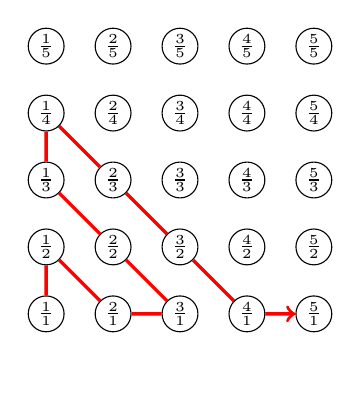
\begin{tikzpicture}[scale=.85,baseline={(0,0)}]
  \foreach \x in {1,...,5}{
    \foreach \y in {1,...,5}{
      \node[circle,inner sep=1pt,draw] (p-\x-\y) at (\x,\y) {\scriptsize $\frac{\x}{\y}$};
    }
  }
  % Zig-zag path (first few steps)
  \draw[very thick,red,->] (p-1-1)--(p-1-2)--(p-2-1)--(p-3-1)--(p-2-2)--(p-1-3)--(p-1-4)--(p-2-3)--(p-3-2)--(p-4-1)--(p-5-1);
  \end{tikzpicture}
  \]
  Skipping repetitions (keep only reduced fractions) we obtain an enumeration of $\mathbb{Q}_{+}$, i.e., an bijection from $\mathbb{Q}_{+}$ to $\N$. Therefore, $|\mathbb{Q}_{+}|=\aleph_0$.
\end{example}


Now let's see some criteria for countability.

\begin{lemma}
  Let $C\subset\N$ be infinite. Then $C$ is countably infinite.
\end{lemma}
\begin{proof}
  Define $f:\N\to C$ inductively as follows: let $f(1)=\min C$. If $f(1),\ldots,f(n)$ have been defined, let $f(n+1)=\min(C\setminus\{f(1),\ldots,f(n)\})$. 

  $f$ is injective: for $m<n$, $f(n)\in C\setminus\{f(1),\ldots,f(n-1)\}$, but $f(m)$ is not in the set. So, $f(n)\neq f(m)$.

  $f$ is surjective: for any $c\in C$, there exists $n\in\N$ such that $f(n)\geq c$. Let $m$ be the smallest integer with $f(m)\geq c$. So for any $i<m$, $f(i)<c$. So $c\notin\{f(1),\ldots,f(m-1)\}$ and hence $f(m)\leq c$ by its definition. This implies that $f(m)=c$.
\end{proof}

The same proof can be used to prove the following result.

\begin{proposition}
If $A$ is infinite, then $|A|\ge \aleph_0$.
\end{proposition}
\begin{proof}
  Since $A$ is infinite, so $A$ is not empty and hence we can choose $\leq$ to make $A$ well-ordered. We define a map $f:\N\to A$ inductive as follows: $f(1)=\min A$. If $f(1),\ldots,f(n)$ have been defined, let $f(n+1)=\min(A\setminus\{f(1),\ldots,f(n)\})$. Then, $f$ is injective. So $|A|\geq \aleph_0$.
\end{proof}

\begin{theorem}
  For any nonempty $A$, the following are equivalent:
  \begin{enumerate}
    \item $A$ is countable;
    \item there exists a surjection $f:\N\to A$;
    \item there exists an injection $g:A\to\N$.
  \end{enumerate}
\end{theorem}
\begin{proof}
  We prove the implications as follows:
  \begin{itemize}
    \item[$(1)\Rightarrow(2)$] If $A$ is countably finite, then there exists a bijection and hence surjection $f:\N\to A$. If $A$ is finite, then the composition is what we need: $\N\to \{1,\ldots,n\}\to A$.
    \item[$(2)\Rightarrow(3)$] If there exists a surjection $f:\N\to A$, then we can define an injection $g:A\to\N$ by $g(a)=\min\{n\in\N:f(n)=a\}$ for all $a\in A$.
    \item[$(3)\Rightarrow(1)$] If there exists an injection $g:A\to\N$, then we can decompose this as $A\to im(g)\to \N$. If $im(g)$ is finite, then $A$ is finite. If $im(g)$ is infinite, then by the lemma above, $im(g)$ is countably infinite and hence so is $A$.
  \end{itemize}
\end{proof}


% \begin{proposition}
% If $A$ is infinite, then $|A|\ge \aleph_0$.
% \end{proposition}
% \begin{proof}
%   Since $A$ is infinite, so $A$ is not empty. We can choose $a_1\in A$. Suppose we have chosen distinct elements $a_1,\ldots,a_n\in A$. Since $A$ is infinite, we can choose another element $a_{n+1}\in A\setminus\{a_1,\ldots,a_n\}$.  Continuing this process, we obtain a sequence of distinct elements \(a_1,a_2,\ldots\) in \(A\).  The map \(f\colon \mathbb{N}\to A\) defined by \(f(n)=a_n\) is an injection, hence \(|A|\geq |\N|=\aleph_0\).
% \end{proof}

% Can we obtain a set \(B\) such that \(|B|>\aleph_0\)?



\begin{theorem}
  The product of finitely many countable sets is countable. 
\end{theorem}

Instead of proving the general theorem, we show a special case.
\begin{proposition}
$|\N\times \N|=\aleph_0$.
\end{proposition}
\begin{proof}
  We can define a function \(f:\N\times\N\to\N\) by
  \[
  f(m,n) = 2^m 3^n.
  \]
  This function is injective, hence $\N\times\N$ is countable. Since $\N\times \N$ is obviously infinite, we have that $|\N\times\N|=\aleph_0$. 
\end{proof}

\fi

% The Fall 2026 Week 2 handout ends with Proposition 1.67.
\ifdefined\stopaftercountableproduct
  \expandafter\endinput
\fi

As a consequence, we have that taking countable unions still cannot increase cardinality.

\begin{theorem}
  Let $A_n$ be a countable set for each \(n\in\N\). Then $\bigcup_nA_n$ is countable.
\end{theorem}
\begin{proof}
  Since $A_n$ is countable, there is a surjection $f_n:\N\to A_n$. Define a function \(f:\N\times \N\to \bigcup_n A_n\) by
  \[
  f(m,n) = f_n(m).
  \]
  This function is surjective, hence \(\bigcup_n A_n\) is countable.
\end{proof}

How about the product of countably many countable sets?

\begin{theorem}
  $\{0,1\}^{\N}$ is uncountable. So the countable product of countable sets need not be countable.
\end{theorem}
\begin{proof}
  Suppose $\{0,1\}^{\N}$ were countable. Then we could list all infinite $0$–$1$ sequences as
  \[
  s^{(1)},s^{(2)},s^{(3)},\ldots,\qquad
  s^{(k)}=(s^{(k)}_1,s^{(k)}_2,s^{(k)}_3,\ldots),\ s^{(k)}_n\in\{0,1\}.
  \]
  Define a new sequence $t=(t_1,t_2,\ldots)$ by flipping the diagonal bits:
  \[
  t_n = 1 - s^{(n)}_n\quad (n\ge 1).
  \]
  Then $t\in\{0,1\}^{\N}$, but $t\neq s^{(k)}$ for every $k$ because they differ in the $k$‑th coordinate. This contradicts the assumption that the list was complete. Hence $\{0,1\}^{\N}$ is uncountable. 
\end{proof}

\newpage

\begin{corollary}
  $|\mathcal{P}(\N)|=|\{0,1\}^{\N}|>|\N|$.
\end{corollary}
\begin{proof}
  Define $\Phi:\{0,1\}^{\N}\to \mathcal{P}(\N)$ by
  \[
  \Phi\bigl((x_n)_{n\ge1}\bigr)=\{\,n\in\N: x_n=1\,\}.
  \]
  If $(x_n)\neq(y_n)$ pick $k$ with $x_k\neq y_k$; then $k$ belongs to exactly one of the two images, so $\Phi(x_n)\neq\Phi(y_n)$. Thus $\Phi$ is injective. Conversely, for any $A\subseteq\N$ let its characteristic sequence $\chi_A$ be given by $\chi_A(n)=1$ if $n\in A$, $0$ otherwise. Then $\Phi(\chi_A)=A$, so $\Phi$ is surjective. Hence $|\mathcal{P}(\N)|=|\{0,1\}^{\N}|$.
\end{proof}

In fact, this corollary is a special case of a more general result which we will prove later.

\begin{theorem}[Cantor's Theorem]
For any set $S$, there is no surjective function from $S$ to its power set $\mathcal{P}(S)$. In particular, $|S| < |\mathcal{P}(S)|$.
\end{theorem}

\begin{corollary}
  $|[0,1)|=|\{0,1\}^{\N}|>\aleph_0$.
\end{corollary}
\begin{proof}
  Define $E\subset \{0,1\}^{\N}$ to be the set of sequences that are not eventually all $1$. Define $\Phi:E\to[0,1)$ by
  \[
  \Phi\bigl((x_n)_{n\ge1}\bigr)=\sum_{n=1}^\infty \frac{x_n}{2^{\,n}}.
  \]
  This is surjective because for any $y\in[0,1)$, we can write $y$ in binary expansion $y=0.y_1y_2y_3\ldots$ with $y_i\in\{0,1\}$ and not ending with an infinite sequence of $1$'s (i.e., when $0.x_1\cdots x_{m-1}1\,0\,0\,0\cdots = 0.x_1\cdots x_{m-1}0\,1\,1\,1\cdots$ happens we choose the expansion that does not end with $1$'s). 
  
  This is also injective: 
  Let $(x_k),(y_k)\in E$ with $(x_k)\ne(y_k)$ and let $n$ be the first index where they differ. WLOG $x_n=0$ and $y_n=1$. Then
  \[
  \Phi(y)-\Phi(x)=\sum_{k=1}^{\infty}\frac{y_k-x_k}{2^k}
  =\frac{1}{2^n}+\sum_{k>n}\frac{y_k-x_k}{2^k}.
  \]
  Since $y_k-x_k\in\{-1,0,1\}$,
  \[
  \sum_{k>n}\frac{y_k-x_k}{2^k}\ge -\sum_{k>n}\frac{1}{2^k}=-\frac{1}{2^n},
  \]
  with equality only if $y_k-x_k=-1$ for all $k>n$, i.e. $x_k=1$ and $y_k=0$ for every $k>n$, which would make $(x_k)$ eventually $1$, contrary to $(x_k)\in E$. Hence the tail sum is strictly greater than $-1/2^n$, so $\Phi(y)-\Phi(x)>0$ and therefore $\Phi(x)\ne\Phi(y)$. 

Therefore, $|[0,1)|=|E|$. Now, we let $D\subset \{0,1\}^{\N}$ be the set of sequences that are eventually $1$. $E=\{0,1\}\setminus D$. We use the following two claims to finish the proof.
  
  \paragraph{Claim 1} $D$ is countable.

  \paragraph{Claim 2} An uncountable set minus a countable set will maintain its cardinality.

  Hence, we have $|E|=|\{0,1\}^{\N}|$. Hence $|[0,1)|=|\{0,1\}^{\N}|>\aleph_0$.

  We will leave Claim 1 as an exercise in your homework 2. We prove Claim 2 below.
\end{proof}


% \begin{proof}
%   For any element $x\in[0,1)$, write by decimals $x=0.a_1a_2a_3\ldots$ with $a_i\in\{0,1,2,\cdots,9\}$. We also make the assumption that the decimal representation does not end with an infinite sequence of 9's, so that $0.999\ldots=1$. So each element has a unique decimal representation.

%   Assume that $[0,1)$ is countable. Then, we can list its elements as $x_1,x_2,\ldots$. Assume that each $x_n$ has the decimal representation $x_n=0.a_{n,1}a_{n,2}a_{n,3}\ldots$. Consider the real number
%   \[
%   y = 0.b_1b_2b_3\ldots
%   \]
%   where $b_n = 3$ if $a_{n,n} \neq 3$, and $b_n = 4$ if $a_{n,n} = 3$. Then $y\in[0,1)$ and $y\neq x_n$ for all $n$, a contradiction.
% \end{proof}


\begin{proposition}
  Let $A$ be an infinite set and $F$ a finite set. Then,
  \begin{itemize}
    \item $|A\cup F|=|A|$.
    \item $|A\setminus F|=|A|$.
  \end{itemize}
  The conclusion still holds if $A$ is uncountable and $F$ is infinitely countable.
\end{proposition}
\begin{proof}
  Let $G:=F\setminus A$. Then $G$ is finite and disjoint from $A$. We need to show that $|A\cup G|=|A|$. Since $A$ is infinite, we can choose a sequence of distinct elements \(a_1,a_2,\ldots\) in \(A\).  If $G=\emptyset$, the result is trivial. If $G\neq\emptyset$, we write $G=\{g_1,g_2,\ldots,g_n\}$, where $n$ is finite. Define $f:A\to A\cup G$ as follows:
  \begin{enumerate}
    \item if $a\notin\{a_1,\ldots\}$, then set $f(a):=a$;
    \item if $a=a_i$ for some $i\leq n$, then set $f(a):=g_i$.
    \item If $a=a_i$ for some $i>n$, then set $f(a):=a_{i-n}$.
  \end{enumerate}
  Then, $f$ is a bijection. Thus $|A\cup G|=|A|$.

  For the second part, we let $B:=A\setminus F$. Then, $|A\setminus F|=|B|=|B\cup (A\cap F)|=|A|$.

  Now, assume that $F$ is countably infinite and $A$ is uncountable. Let $G:=F\setminus A$. Then, $G$ is countable. WLOG, we assume $G$ is infinite. We then can write $G=\{g_1,g_2,\ldots\}$. Still choose a sequence of distinct elements \(a_1,a_2,\ldots\) in \(A\). Define $f:A\to A\cup G$ as follows:
  \begin{enumerate}
    \item if $a\notin\{a_1,\ldots\}$, then set $f(a):=a$;
    \item if $a=a_{2n}$, then set $f(a_{2n}):=g_n$;
    \item if $a=a_{2n-1}$, then set $f(a_{2n-1}):=a_{n}$.
  \end{enumerate}
  Then, $f$ is a bijection. Thus $|A\cup G|=|A|$.

\end{proof}

\begin{corollary}
  $|[0,1)|=|[0,1]|=|(0,1)|=|(0,1]|$.
\end{corollary}

\begin{proposition}
  $|(0,1)|=|\mathbb{R}|$.
\end{proposition}
\begin{proof}
  Let $f:(0,1)\to\mathbb{R}$ be defined by
  \[
  f(x) = \tan\bigl((x-\tfrac{1}{2})\pi\bigr).
  \]
  Then $f$ is a bijection, hence $|(0,1)|=|\mathbb{R}|$.
\end{proof}

\begin{corollary}
  $|\R\setminus\Q|=|\R|$.
\end{corollary}






\subsubsection{Proofs of some general theorems}

\begin{theorem}[Cantor-Schröder-Bernstein]
If there exist injections \(f: A \to B\) and \(g: B \to A\), then there exists a bijection \(h: A \to B\).
\end{theorem}
\begin{proof}
WLOG, we assume that $A$ and $B$ are disjoint (otherwise replace $B$ by a disjoint copy). For each $a\in A$, we have the following sequence:
\[\ldots\overset{f}{\mapsto} b_{-3}\overset{g}{\mapsto} a_{-2}\overset{f}{\mapsto} b_{-1}\overset{g}{\mapsto} a_0=a\overset{f}{\mapsto} b_0\overset{g}{\mapsto} a_1\overset{f}{\mapsto} b_1\overset{g}{\mapsto} a_2\overset{f}{\mapsto} \ldots\]
There are only four possibilities for this sequence:
\begin{enumerate}
  \item ($B$-stopper) it stops at some $b_{-k}$ where $k\geq 1$. 
  \item ($A$-stopper) it stops at some $a_{-k}$ where $k\geq 0$.
  \item (bi-infinite) it continues indefinitely in both directions.
  \item (cyclic) it is a cyclic sequence, i.e., $a_i=a_j$ for some $i<j$.
\end{enumerate}

This also holds for any $b\in B$ and hence these four possibilities give rise to a partition of $A\sqcup B$.

Now, we define $h:A\to B$ as follows:
\[
h(a) =
\begin{cases}
f(a), & \text{if $a$ is an $A$-stopper};\\
f(a), & \text{if $a$ is in a bi-infinite chain or a cycle};\\
g^{-1}(a), & \text{if $a$ is a $B$-stopper}.
\end{cases}
\]

This is a bijection.
\end{proof}


We proved this using Well-ordering theorem. We can also prove this using Zorn's lemma.
\begin{theorem}
If $A,B$ are sets then either $|A|\le |B|$ or $|B|\le |A|$.
\end{theorem}

\begin{proof}
Let $\mathcal{M}$ be the set of \emph{matchings} between $A$ and $B$:
\[
\mathcal{M} = \{ M \subseteq A \times B \mid \text{each } a \in A \text{ appears in at most one pair of } M, \ \text{and each } b \in B \text{ appears in at most one} \}.
\]
We partially order $\mathcal{M}$ by inclusion.  
If $\{ M_i \}_{i \in I}$ is a chain in $\mathcal{M}$, then
\[
M = \bigcup_{i \in I} M_i
\]
is again a matching, since no element of $A$ or $B$ can be matched to more than one partner within a chain. Thus every chain has an upper bound.

By \emph{Zorn's Lemma}, $\mathcal{M}$ has a maximal element $M^\ast$.

Suppose there exist $a \in A$ and $b \in B$ both unmatched in $M^\ast$. Then
\[
M' = M^\ast \cup \{ (a,b) \}
\]
is a matching strictly larger than $M^\ast$, contradicting maximality. Therefore, at least one side is fully matched: either every $a \in A$ is matched, or every $b \in B$ is matched.

\begin{itemize}
    \item If every $a \in A$ is matched, define $f: A \to B$ by $f(a) = b$ whenever $(a,b) \in M^\ast$. This $f$ is injective, so $|A| \le |B|$.
    \item Otherwise, every $b \in B$ is matched. Define $g: B \to A$ by $g(b) = a$ whenever $(a,b) \in M^\ast$. Then $g$ is injective, so $|B| \le |A|$.
\end{itemize}

Thus, for any sets $A$ and $B$, either $|A| \le |B|$ or $|B| \le |A|$.
\end{proof}

\begin{theorem}[Cantor's Theorem]
For any set $S$, there is no surjective function from $S$ to its power set $\mathcal{P}(S)$. In particular, $|S| < |\mathcal{P}(S)|$.
\end{theorem}

\begin{proof}
Suppose $f\colon S\to \mathcal{P}(S)$ is any function. Define $B = \{s \in S : s \notin f(s)\}$. If $B\subseteq S$ is in the range of $f$, then there exists $s_0 \in S$ such that $f(s_0) = B$. The following contradictions arise: one can show that
\[s_0\in B \implies s_0\notin f(s_0) = B \quad\text{and}\quad s_0\notin B = f(s_0) \implies s_0\in B,\]
which forces a contradiction. Consequently any function $f\colon S\to \mathcal{P}(S)$ must fail to be surjective, and hence $|S|\neq |\mathcal{P}(S)|$. On the other hand, there is an obvious injection $S\to \mathcal{P}(S)$ given by $s\mapsto\{s\}$. Therefore
\[|S| < |\mathcal{P}(S)|<|\mathcal{P}(\mathcal{P}(S))|<\dots.
\]
\end{proof}

%---------------------------------------------------------------------------

\newpage
